%Created: 2023-08-20
%By: VictorieeMan
%URL: https://github.com/VictorieeMan/KTH-KF1050-kompendium

% ------------------- %

%basic preamble
\documentclass[11pt,a4paper]{article}
\usepackage[utf8]{inputenc}
\usepackage[swedish]{babel}
\usepackage{amsmath}
\usepackage{amssymb}

%custom timestamp
\usepackage[yyyymmdd]{datetime}
	\renewcommand{\dateseparator}{--}

%QR-code
\usepackage{qrcode}

%URL
\usepackage{hyperref}

% Tikz
\usepackage{tikz}
\usetikzlibrary{shapes.geometric, arrows}

%Variables
\newcommand{\pdfUrl}{https://github.com/VictorieeMan/KTH-KF1050-kompendium/releases}
\newcommand{\email}{\texttt{kontakt.fvjjg@e-mail.victoriee.org}}

% ------------------- %

% Titlepage
\title{Polymera Material\\KTH:KF1050-kompendium}
\author{Victor Ekekrantz}

% ------------------- %

% Document
\begin{document}

\pagenumbering{gobble}
\maketitle

\selectlanguage{swedish}
\section*{Förord}
%qr code to the repo url
Senaste versionen av detta kompendium finns att hämta på:\\
\url{\pdfUrl}\\
\qrcode[height=1in]{\pdfUrl}\\


\noindent
Kontakt: \email

\noindent
Kompileringstid:\\ %\pdfcreationdate
\noindent
Date: \today,\ Time: \currenttime
\tableofcontents

\pagenumbering{arabic}
\selectlanguage{swedish}
\section{Förkunskaper}
\subsection{Kemi}
Kemiska reaktioner, jämviktsreaktioner, kemiska beteckningar och beräkningar, kovalenta bindningar, van der waals krafter, joner, lösningar, kolväten, estrar, alkener, styren, polär
\subsection{Hållfasthet}
\selectlanguage{swedish}
\section{Polymerer}
%Grundläggande polymerkemi och vad som är gemensamt för allt inom materialgruppen och studien av polymerer.
Polymera material består utav polymer kedjor. Dessa kedjor är uppbyggda av repeteradne enheter av monomerer. Monomerer är den minsta repeterande enheten i en polymerkedja. Processen som kopplar samman monomerer till polymerkedjor är benämnd polymerisering.

\begin{figure}[ht]
    \centering
    % Träddiagram av polymertyperna:
%Ref: PolyT p. 5
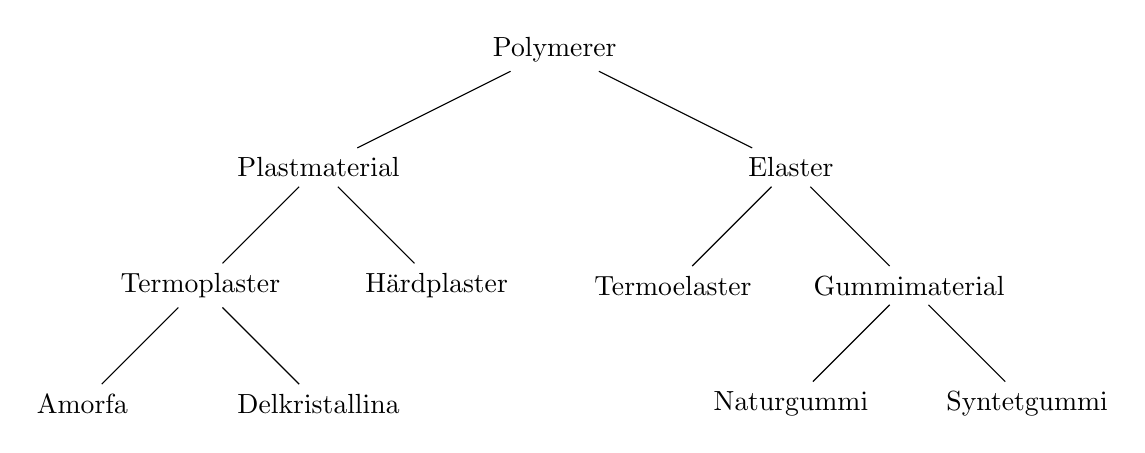
\begin{tikzpicture}[
    level 1/.style={sibling distance=6cm},
    level 2/.style={sibling distance=3cm},
    level 3/.style={sibling distance=3cm}
  ]
    \node {Polymerer}
        child { node {Plastmaterial}
            child { node {Termoplaster} 
                child { node {Amorfa} }
                child { node {Delkristallina} }    
            }
            child { node {Härdplaster} }
        }
        child { node {Elaster}
            child { node {Termoelaster} }
            child { node {Gummimaterial} 
                child { node {Naturgummi} }
                child { node {Syntetgummi} }
            }
        };
\end{tikzpicture}

    \caption{Kategorisering av polymertyper \cite[s.5]{polym}}
    \label{fig:polymer_typer}
\end{figure}

% %Beskrivning av skiljelinjen mellan plastmaterial och elaster.
% \subsection{Plaster}
% %Grundläggande om plastmaterial och deras egenskaper.
% \subsection{Elaster}
% %Grundläggande om elaster och deras egenskaper.

% \subsection{Naturliga polymerer}
% \subsection{Kommersiella polymerer}
% \subsection{Komposit material}

\subsection{Plaster och Elaster}
\subsubsection{Naturliga polymerer}
\subsubsection{Kommersiella polymerer}

\subsection{Molekylstrukturen}
\subsubsection{Molekylvikt}
\subsubsection{Konfiguration}
\subsubsection{Konformation}

\subsection{Mikrostrukturen}
%Amorf, delkristalina
\include{input/modules/polymerstrukturen}
% \section{Plaster}
%Grundläggande om plastmaterial och deras egenskaper.

%Termoplaster
%%Amorfa
%%Delkristalina

%Härdplaster

\section{Termoplaster}
\subsection{Amorfa}
% Content about amorphous thermoplastics

\subsection{Delkristallina}
% Content about crystalline thermoplastics

\section{Härdplaster}
% Content about thermosetting plastics
\selectlanguage{swedish}
% \section{Elaster}
%Grundläggande om elaster och deras egenskaper.

%Termoelaster
%Gummimaterial
%%Naturgummi
%%Syntetgummi

\section{Termoelaster}
% Content about thermoplastic elastomers

\section{Gummimaterial}
\subsection{Naturgummi}
% Content about natural rubber

\subsection{Syntetgummi}
% Content about synthetic rubber
\include{input/modules/mekaniska_egenskaper}
\selectlanguage{swedish}
\section{Polymerisering}
Den syntetiska processen att länka samman monomerer till polymera kedjor, kallas för polymerisation. Detta kan göras genom olika typer utav kem\-iska mekanismer, vilka kan delas in i fyra kategorier: Stegvis.., Kedjevis.., Ringöpnings.. och övriga polymerisationstekniker \cite[s. 117]{polym}.

Oavsett teknik så handlar polymerisation om att monomerer kopplas samman till polymerer. Detta sker genom att monomerer adderas till en växande polymerkedja. Detta kan ske på två sätt: antingen genom att en monomer adderas i taget, eller genom att flera monomerer adderas samtidigt. I det första fallet talar vi om stegvis polymerisation, och i det andra fallet talar vi generellt om kedjevis polymerisation.

Vårt huvudfokus kommer att ligga på stegvis polymerisation och kedjevis polymerisation, två helt olika processer som är mycket vanliga ute i industrin \cite[s. 131]{polym}. Notera att kedjevis polymerisation är ett samlingsnamn för tre principiellt liknande processer: radikal.., jon.. och koordinationspolymerisation. Trädet nedan visualiserar den beskrivna kategoriseringen av polymerisationstekniker.

\begin{figure}[ht]
    \centering
    % Träddiagram av polymeriserings typerna:
%Ref: PolyT p. 117
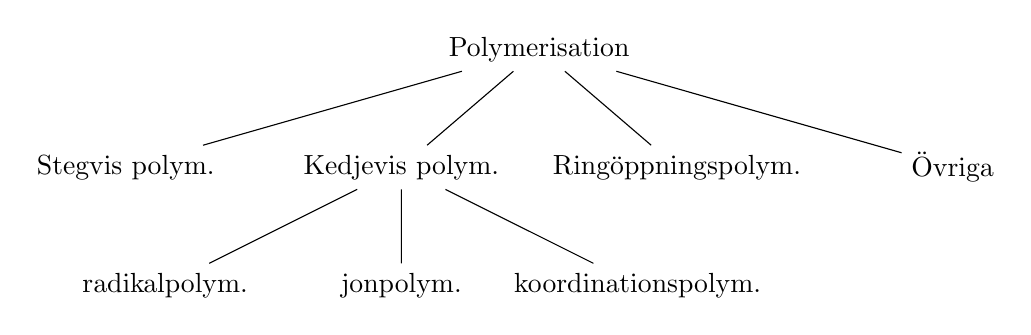
\begin{tikzpicture}[
    level 1/.style={sibling distance=3.5cm},
    level 2/.style={sibling distance=3cm},
    level 3/.style={sibling distance=3cm}
  ]
    \node {Polymerisation}
        child { node {Stegvis polym.}
        }
        child { node {Kedjevis polym.}
            child { node {radikalpolym.} }
            child { node {jonpolym.} }
            child { node {koordinationspolym.} }
        }
        child { node {Ringöppningspolym.}
        }
        child { node {Övriga}
        };
\end{tikzpicture}
    \caption{Kategorisering av polymerisationstekniker \cite[s.117]{polym}}
    \label{fig:polymerisations_typer}
\end{figure}

Polymeriseringsprocesser
\subsection{Stegvis polymerisation}
%Ethene chemfig



\subsection{Kedjevis polymerisation}
\subsubsection{Radikalpolymerisation}
\subsubsection{Jonpolymerisation}
\subsubsection{Koordinationspolymerisation}
\subsection{Ringöppningspolymerisation}
\subsection{Övriga polymerisationstekniker}

\selectlanguage{swedish}
\section{Produktion \& Livscykel}
%Framställning
%Additiv
%Form och bearbetning
\subsection{Additiv}
\subsection{Form och bearbetning}
\subsection{Kassering och Återvinning}
% \include{input/modules/livscykel}
% \include{input/modules/återvinning}

\pagenumbering{roman}
% Källor och referenser
\begin{thebibliography}{0}
    \bibitem{polym}
    Polymerteknologi -- Makromolekylär design; Ann-Christine Albertsson, Ulrica Edlund, Karin Odelius; Stockholm 2022; ISBN: 978-91-7415-449-8
\end{thebibliography}

\include{input/modules/draft}

\end{document}